\section{Results}

\lulu{lulu to write}

\label{sec:Discussion}

\subsection{Implementation Details}

Experiments are ran on L40S GPUs. 

\subsection{Datasets}
We evaluate our method on the iPhone~\cite{gao2022dynamic} dataset and the Nvidia~\cite{yoon2020novel} dataset. The iPhone dataset consists of 14 casually captured videos, 7 of which contains test camera views. We evaluate on 5 of those 7 views as the remaining two have camera inaccuracies, following \cite{wang2025shape}. The Nvidia dataset contains 7 scenes shot with static cameras of multiple views. \todo{We also show qualitative results from the DAVIS dataset}. 
% Was an inline wrapfigure in sec/5_results.tex (workshop version); captions = its commented-out captions.
\begin{figure}[t]
  \centering
  \begin{subfigure}[b]{0.49\linewidth}
    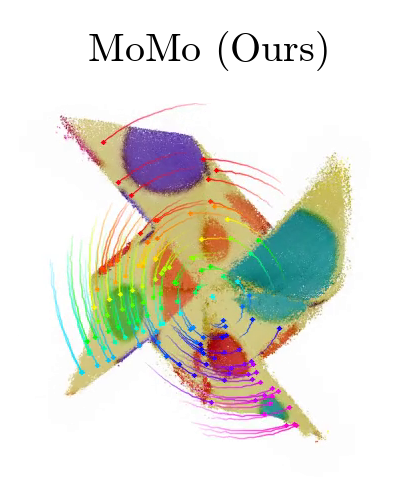
\includegraphics[width=\linewidth]{img/ours-tracks}
    \caption{Ours}
  \end{subfigure}
  \hfill
  \begin{subfigure}[b]{0.49\linewidth}
    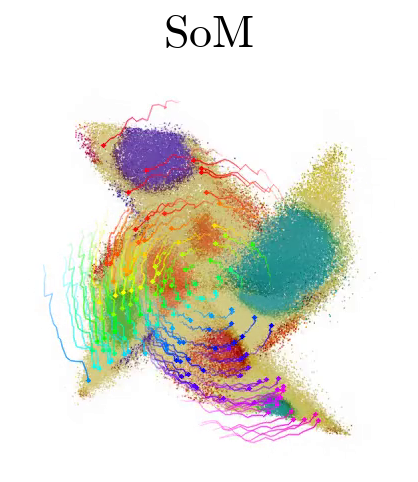
\includegraphics[width=\linewidth]{img/som-tracks}
    \caption{Shape of Motion}
  \end{subfigure}
  \caption{\lulu{Update with new MoMo} Comparison of estimated 3D tracks.}
  \label{fig:synthetic-tracks}
\end{figure}

For the synthetic pinwheel scene, we show tracks obtained from SoM~\cite{wang2025shape} and our method.
SoM-produced tracks display jitters across the tracks, while our method faithfully recovers the main rotational motion.

% fig/qualitative_comparison.tex is input at the top of sec/4_method.tex (two-column float; from here it would land after the references)
%We report quantitative and qualitative results on the DyCheck~\cite{gao2022dynamic} dataset, comparing against SoM~\cite{wang2025shape} as our main baseline, using \todo{PSNR, LPIPS, and SSIM} to evaluate image quality.
% \begin{table*}[t]
  \centering
  \definecolor{rowgray}{gray}{0.9}
  \setlength{\tabcolsep}{4.5pt}
  \renewcommand{\arraystretch}{1.25}
  \begin{tabular}{@{}lcccccc@{}}
    \toprule
    \textbf{Scene}
      & \shortstack{\textbf{PSNR\,$\uparrow$}\\ \textbf{SoM}} & \shortstack{\textbf{PSNR\,$\uparrow$}\\ \textbf{Ours}}
      & \shortstack{\textbf{SSIM\,$\uparrow$}\\ \textbf{SoM}} & \shortstack{\textbf{SSIM\,$\uparrow$}\\ \textbf{Ours}}
      & \shortstack{\textbf{LPIPS\,$\downarrow$}\\ \textbf{SoM}} & \shortstack{\textbf{LPIPS\,$\downarrow$}\\ \textbf{Ours}} \\
    \midrule
    \rowcolor{rowgray}
    apple          & \textbf{11.99} & 11.19          & 0.9890 & \textbf{0.9894} & 0.2299          & \textbf{0.2298} \\
    paper-windmill & 11.72          & \textbf{12.15} & 0.9723 & \textbf{0.9733} & 0.4471          & \textbf{0.4173} \\
    \rowcolor{rowgray}
    teddy          & \textbf{12.56} & 12.33          & 0.7281 & \textbf{0.7297} & \textbf{0.4630} & 0.4842          \\
    \textbf{Average} & \textbf{12.09} & 11.89        & 0.8965 & \textbf{0.8975} & 0.3800          & \textbf{0.3771} \\
    \bottomrule
  \end{tabular}
  \caption{Quantitative comparison against Shape-of-Motion (SoM)~\cite{wang2025shape} on the Apple, Paper Windmill, and Teddy scenes from the DyCheck dataset. Best result per metric is shown in \textbf{bold}.}
  \label{tab:quantitative}
\end{table*}

% \begin{table*}[t]
  \centering
  \definecolor{rowgray}{gray}{0.9}
  \setlength{\tabcolsep}{4.5pt}
  \renewcommand{\arraystretch}{1.25}
  \begin{tabular}{@{}lcccccc@{}}
    \toprule
    \textbf{Scene}
      & \shortstack{\textbf{PSNR\,$\uparrow$}\\ \textbf{SoM}} & \shortstack{\textbf{PSNR\,$\uparrow$}\\ \textbf{Ours}}
      & \shortstack{\textbf{SSIM\,$\uparrow$}\\ \textbf{SoM}} & \shortstack{\textbf{SSIM\,$\uparrow$}\\ \textbf{Ours}}
      & \shortstack{\textbf{LPIPS\,$\downarrow$}\\ \textbf{SoM}} & \shortstack{\textbf{LPIPS\,$\downarrow$}\\ \textbf{Ours}} \\
    \midrule
    \rowcolor{rowgray}
    apple          & 11.99 & \todo{\textbf{12.01}}          & 0.9890 & \textbf{0.9902} & 0.2299          & \textbf{0.2214} \\
    paper-windmill & 11.72          & \todo{\textbf{12.08}} & 0.9723 & \textbf{0.9727} & 0.4471          & \textbf{0.4195} \\
    \rowcolor{rowgray}
    \todo{teddy}          & \textbf{12.56} & 12.33          & 0.7281 & \textbf{0.7297} & \textbf{0.4630} & 0.4842          \\
    \todo{\textbf{Average}} & \textbf{12.09} & 11.89        & 0.8965 & \textbf{0.8975} & 0.3800          & \textbf{0.3771} \\
    \bottomrule
  \end{tabular}
  \caption{\todo{TMP - newer results after changes} Quantitative comparison against Shape-of-Motion (SoM)~\cite{wang2025shape} on the Apple, Paper Windmill, and Teddy scenes from the DyCheck dataset. Best result per metric is shown in \textbf{bold}.}
  \label{tab:quantitative}
\end{table*}


We also provide qualitative results on the DyCheck~\cite{gao2022dynamic} benchmark (Fig.~\ref{fig:qualitative-comparison}. 
At the same number of bases ($B=20$), our method achieves higher reconstruction quality than SoM, with strong regularization still holding at this basis count, while SoM shows clear overfitting and degraded test-view quality. In the `Paper Windmill' scene specifically, a real video version of our synthetic example, the recovered Gaussian tracks show our method preserving the dominant windmill-rotation motion, while SoM produces per-Gaussian overfitted tracks that fail to capture this coherent motion.

% fig/tab_full_dycheck.tex and fig/tab_full_nvidia.tex are input in the supplementary, sec/X_suppl.tex ([Claude] 2026-11-05, user request)
% [Claude] 2026-11-05: motion-coefficient comparison moved up from the end of the section, before the line plots (user request).
% [Claude] 2026-10-28: placeholder for the motion-coefficient comparison (user request); grey boxes stand in for the images.
% [Claude] 2026-11-05 (user requests): apple (seed 44), Balloon1 (seed 43) and teddy (seed 43) at the first training frame (0_00000), spin (seed 42)
% at training frame 0_00270 (18 s into the 15 fps render). Coefficients = that frame of tests/render_coefs.py's renders (outputs/bdf/modes_vis/
% {som/<S>/bases_10,split_init/<S>/bases_<B>}[_s<seed>]/videos/epoch_0499/motion_coefs.mp4, right half); input = the dataset's training image,
% cropped like the render (Balloon1: 458 x 240 of 470 x 248; DyCheck 720 x 960, uncropped).
\begin{figure}[t]
  \centering
  \newcommand{\coefrow}[3]{\rotatebox{90}{\makebox[#2\linewidth][c]{\footnotesize #3}} & \coefimg{coef_#1_input} & \coefimg{coef_#1_som10} &
    \coefimg{coef_#1_ours} \\}
  \newcommand{\coefimg}[1]{\includegraphics[width=0.3\linewidth]{img/#1}}
  \setlength{\tabcolsep}{1pt}
  \begin{tabular}{@{}c@{\hspace{2pt}}ccc@{}}
    \coefrow{apple_s44_f0}{0.4}{Apple}
    \coefrow{Balloon1_s43_f0}{0.157}{Balloon1}
    \coefrow{teddy_s43_f0}{0.4}{Teddy}
    \coefrow{spin_s42_f270}{0.4}{Spin}
     & \makebox[0.3\linewidth][c]{\footnotesize Input} &
       \makebox[0.3\linewidth][c]{\footnotesize SoM-10} &
       \makebox[0.3\linewidth][c]{\footnotesize Ours} \\
  \end{tabular}
  \caption{\claudetag\ Motion coefficients of Shape of Motion~\cite{wang2025shape} with its default 10 bases and of our method
    ($B$ from its stopping rule: 5 on apple, 4 on Balloon1, 8 on teddy, 9 on spin), rendered from a training view: the first one for
    apple (DyCheck, seed 44), Balloon1 (NVIDIA, seed 43) and teddy (DyCheck, seed 43), frame 270 for spin (DyCheck, seed 42). Each
    foreground Gaussian is coloured by its blending weights: every basis of a model has its own hue, spaced evenly over that model's
    bases, and mixed weights mix the hues; the background is grey. Hues are not matched between the two methods: what matters is which
    parts share one colour.}
  \label{fig:coef-comparison}
\end{figure}

\Cref{fig:coef-comparison} compares the motion coefficients of Shape of Motion and our method.
\todo{discuss once the images exist.}

% Claude, generated by tests/plot_som_sweep_iphone.py --average --scenes apple teddy spin paper-windmill block --name iphone_avg
% (branch bd-split-rules): SoM rerun on the current code (seed 42, B = 1..10) averaged over the five iPhone scenes at each B; ours
% (seed 42) at the mean of its per-scene B (apple 5, teddy 8, spin 9, paper-windmill 9, block 7); open circle = SoM averaged at
% each scene's B.
% [Claude] 2026-11-05 (user request): validation only, one panel per dataset, Fig. 2b style, MoMo final (split_init at the tables' B:
% DyCheck 5 8 9 9 10, NVIDIA 4 6 8 7 5 6 6). tests/plot_sweep_val_avg.py -> plots/sweep_val_avg/sweep_val_{dycheck,nvidia}.pdf (copied to img/).
% Seed 42, last epoch, val/fg_psnr. DyCheck SoM sweep: outputs/bdf/som; NVIDIA SoM sweep: the Killarney sweep (outputs/bdf_nvsweep, parity
% with Vulcan within 0.1 dB). Values: DyCheck MoMo 12.64 at B 8.2, SoM at each B 12.64, SoM-10 12.63, SoM peak 12.74 at B 3;
% NVIDIA MoMo 20.42 at B 6.0, SoM at each B 20.19, SoM-10 20.32, SoM max 20.38 at B 9.
\begin{figure}[t]
  \centering
  \begin{subfigure}{\linewidth}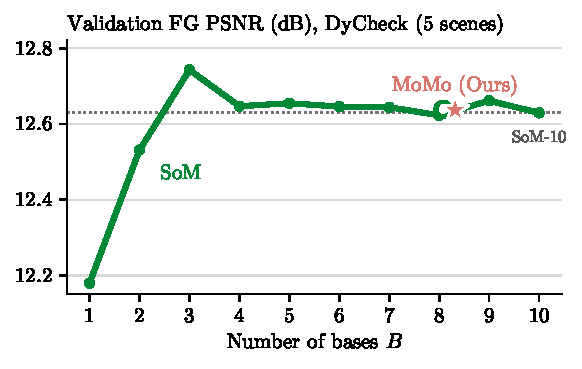
\includegraphics[width=\linewidth]{img/sweep_val_dycheck.pdf}\phantomsubcaption\label{fig:sweep-avg-dycheck}\end{subfigure}\\[2pt]
  \begin{subfigure}{\linewidth}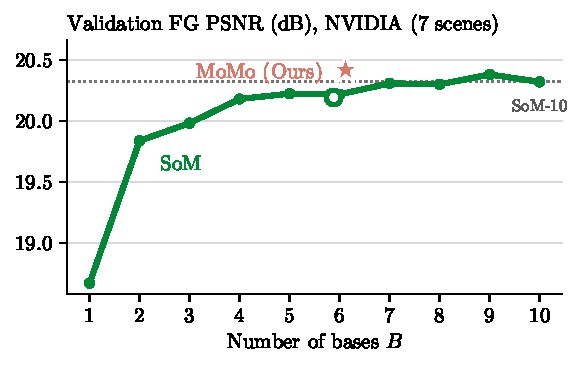
\includegraphics[width=\linewidth]{img/sweep_val_nvidia.pdf}\phantomsubcaption\label{fig:sweep-avg-nvidia}\end{subfigure}
  \caption{\claudetag\ Foreground PSNR on the held-out views against the number of bases, averaged over the five DyCheck
    (iPhone) scenes (top) and the seven NVIDIA scenes (bottom): SoM~\cite{wang2025shape} with $B = 1$--$10$ bases (curve), ours at
    the mean of the $B$ its stopping rule picks per scene (star; 8.2 on DyCheck, 6.0 on NVIDIA) and SoM given each scene's $B$
    (circle); dotted line: SoM-10. Seed 42.}
  \label{fig:sweep-avg}
\end{figure}

% % Claude, generated by tests/plot_track_error_vs_bases.py --average (branch bd-split-rules): track error (masked L1, SoM's track
% loss) of the initialisation, before photometric training, seed 42, mean over apple, teddy, spin, paper-windmill and block.
% SoM init (k-means + Procrustes + 1000 Adam iterations) at B = 1..10; MoMo with its own 5 % rule (B = 6, 9, 9, 6, 7).
\begin{figure}[t]
  \centering
  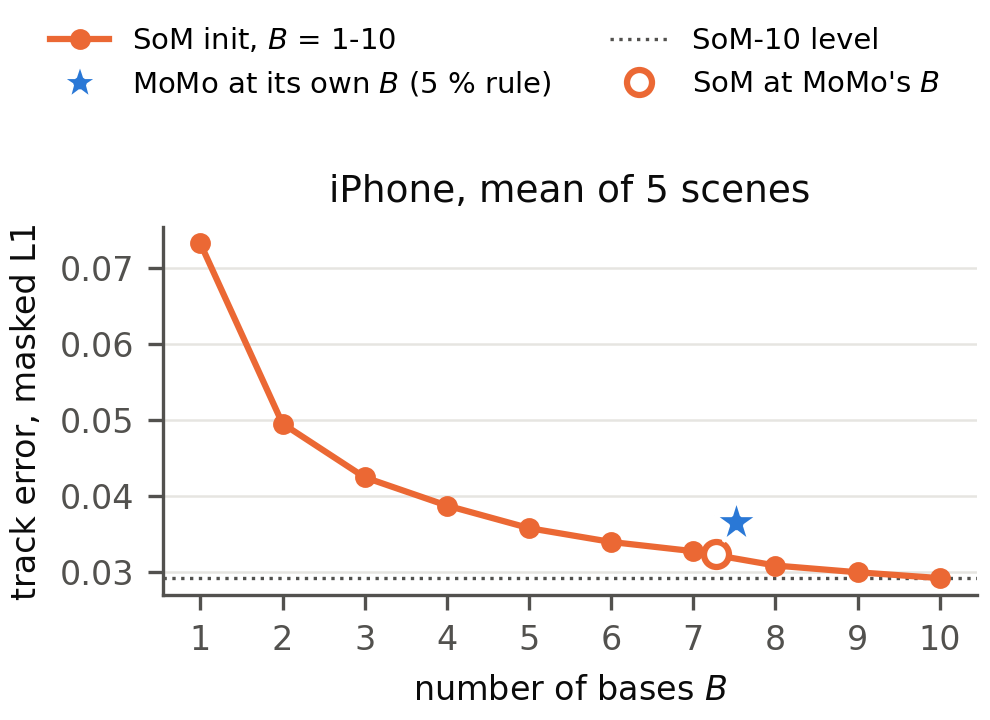
\includegraphics[width=\linewidth]{img/track_error_iphone_avg.png}
  \caption{\claudetag\ \claudeadd{Track error of the initialization (masked $\ell_1$ distance to the 3D tracks, before photometric
    training) against the number of bases, averaged over the five DyCheck (iPhone) scenes: SoM~\cite{wang2025shape} with
    $B = 1$--$10$ bases (curve), MoMo with the number of bases its $\tau = 0.05$ cutoff chooses (star) and SoM with that same number
    (circle); dotted line: SoM-10. Lower is better. Seed 42.}}
  \label{fig:track-avg}
\end{figure}
   % [Claude] 2026-11-05: Fig. 6 (track error vs. number of bases) removed (user request); the file is kept
% [Claude] 2026-11-04: inside the pending \claudedel below, \todo{...} became \textcolor{red}{TODO:} + plain text, because \sout cannot break a braced argument and the line ran 107pt into the margin; same words.
\Cref{tab:full-dycheck,tab:full-nvidia} compare our method (\cref{sec:split-init}) on the full held-out views with SoM~\cite{wang2025shape}
at its default 10 bases (SoM-10) and with as many bases as ours (SoM-$B$). On DyCheck, with
8.2 bases on average, ours is level with both in PSNR ($-0.01$\,dB against SoM-$B$, $-0.03$\,dB against SoM-10) and ahead in
LPIPS ($-0.003$ and $-0.002$) and SSIM. On NVIDIA, with 6.0 bases on average, ours is again level, $+0.01$\,dB against SoM-$B$ and
$-0.02$\,dB against SoM-10 with an LPIPS 0.002 higher: it is ahead on Truck ($+0.20$\,dB against SoM-10) and Umbrella ($+0.02$\,dB) and
behind SoM-10 by 0.03--0.12\,dB on the other five scenes. The residual-pattern clustering is what makes the coefficients separate the
moving parts (one basis per person in Jumping, the toy's legs in teddy); without it (movers = the whole poorly fitted half,
$\ell_1$ residual) the coefficients blend neighbouring parts, at $+0.07$\,dB PSNR on DyCheck and $+0.02$\,dB on NVIDIA
(paired over 13 and 20 runs).
\Cref{fig:sweep-avg} averages the trade-off over the scenes of each
dataset, on the held-out views (foreground PSNR, seed 42). On DyCheck, SoM peaks at 12.74\,dB at three bases and stays near 12.65\,dB
from then on (12.63\,dB at ten); ours, at 8.2 bases on average, scores 12.64\,dB, level with SoM given each scene's number of bases
(12.64\,dB) and with SoM-10. On NVIDIA, SoM rises to 20.2--20.4\,dB from four bases on (20.32\,dB at ten); ours, at 6.0 bases on
average, scores 20.42\,dB, above SoM given each scene's number of bases (20.19\,dB) and SoM-10.
% [Claude] 2026-11-05 (user request): Fig. 2b on the real scenes. tests/plot_scene_avg_coef.py -> plots/scene_avg_coef/avg_blending_weight_
% {nvidia,dycheck}_sorted.pdf (copied to img/): average softmax blending weight per basis, ours (split_init at the tables' B) vs SoM-10, mean over
% seeds 42-44 (block SoM: 42 / 43), each run's bases sorted by weight; rank k averaged over the scenes that have it (ours: NVIDIA 7 7 7 7 6 5 2 1,
% DyCheck 5 5 5 5 5 4 4 4 3 1). Curves: NVIDIA ours 0.372 0.244 0.174 0.104 0.070 0.043 0.037 0.034, SoM-10 0.190 0.158 0.133 0.112 0.097 0.087
% 0.074 0.058 0.050 0.042; DyCheck ours 0.375 0.183 0.123 0.087 0.072 0.069 0.054 0.042 0.037 0.038, SoM-10 0.182 0.146 0.122 0.111 0.102 0.087
% 0.075 0.068 0.060 0.046 (top values to 4 decimals: 0.3719 / 0.1897 NVIDIA, 0.3746 / 0.1824 DyCheck).
% [Claude] 2026-11-05: NVIDIA panel switched from native to sorted order (user request), restored after a concurrent edit reverted it.
\begin{figure}[t]
  \centering
  \begin{subfigure}{\linewidth}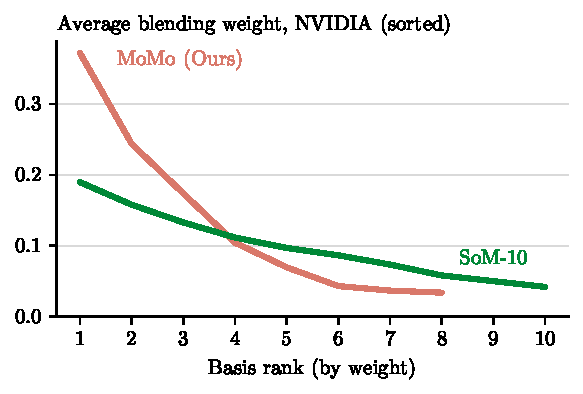
\includegraphics[width=\linewidth]{img/avg_blending_weight_nvidia_sorted.pdf}\phantomsubcaption\label{fig:avg-weight-nvidia}\end{subfigure}\\[2pt]
  \begin{subfigure}{\linewidth}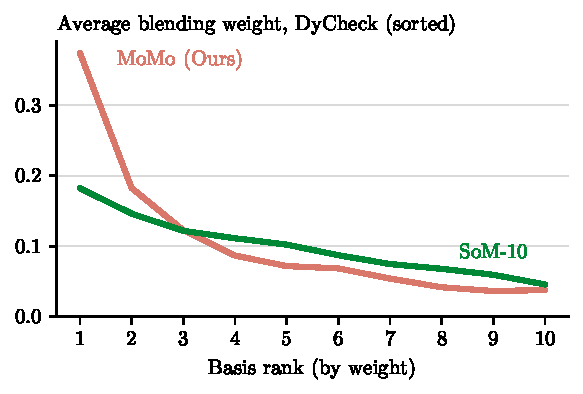
\includegraphics[width=\linewidth]{img/avg_blending_weight_dycheck_sorted.pdf}\phantomsubcaption\label{fig:avg-weight-dycheck}\end{subfigure}
  \caption{Average blending weight of each basis on the real scenes: ours with the
    $B$ its stopping rule picks per scene against SoM~\cite{wang2025shape} with its default 10 bases (SoM-10), mean over three seeds and
    over the scenes, with each model's bases sorted by weight, which does not depend on SoM's arbitrary basis order. Top: the seven
    NVIDIA scenes. Bottom: the five DyCheck scenes. A rank is averaged over the scenes that have it, so ours ends at the largest $B$ of
    the dataset.}
  \label{fig:avg-weight-real}
\end{figure}

\Cref{fig:avg-weight-real} shows the average blending weight of each basis on the real scenes. Ours concentrates the weight on
few bases: with the bases sorted by weight, its strongest basis carries 0.37 of the weight on both datasets, against 0.19 (NVIDIA) and
0.18 (DyCheck) for SoM-10, and its three strongest carry 0.79 and 0.68 against 0.48 and 0.45.
We compare the two initializations on the 3D tracks alone, % [Claude] 2026-11-05: the struck reference was \Cref, written as Fig.~\ref because \sout cannot process \cref
 with MoMo choosing its number of bases by the
$\tau = 0.05$ cutoff (6, 9, 9, 6 and 7 bases on apple, teddy, spin, paper-windmill and block; 7.4 on average). MoMo's initialization does
not fit the tracks more tightly than SoM's: at the same number of bases its masked $\ell_1$ track error is 13\,\% higher on
average and higher on every scene. Trained with these $B$ (seed 42), MoMo reaches 16.75\,dB PSNR on the held-out views on average, 0.08\,dB below SoM
given the same $B$ and 0.06\,dB below SoM-10, with a slightly lower LPIPS (0.386 against 0.388 and 0.390); the gap is
within the seed spread and comes mostly from spin. On NVIDIA the $\tau$ cutoff chooses 5.6 bases on average (5, 4, 9, 6, 5, 4 and 6 on
Balloon1, Balloon2, Jumping, Playground, Skating, Truck and Umbrella); the initialization's track error is again higher than
SoM's at the same $B$ (by 14\,\% on average and on every scene), yet after training MoMo is 0.11\,dB above SoM given the same
$B$ (23.37 against 23.26\,dB) and 0.03\,dB below SoM-10 (23.40\,dB), with LPIPS 0.101 against 0.102 and 0.100.
\Cref{tab:full-dycheck,tab:full-nvidia} use, for each scene, the $B$ the $\tau = 0.05$ cutoff picks with the current initialization (seed 42).

% [Claude] 2026-10-28: comparison with prior work, placeholder (user request); table in fig/tab_sota_nvs.tex.
% [Claude] 2026-10-28: placeholder comparison with prior work on novel view synthesis, laid out like MotionScale's table (user
% screenshot), ours as the last row. Only our own runs (user 2026-10-28): Shape of Motion = our SoM-10 reruns and ours = the candidate
% default, both the average rows of fig/tab_full_{dycheck,nvidia}.tex (DyCheck: 4 of 5 scenes, block pending). MoSca trained but was not
% scored, Gaussian Marbles / HiMoR training crashed (missing LPIPS alex.pth), MotionScale not run: TODO.
% [Claude] 2026-11-05: Ours re-synced with those average rows, which are MoMo (L2 + clustering + 5 % cutoff, user 2026-11-04) since
% 2026-11-04; this row still held the old MoMo (energy + L1). NVIDIA now includes Umbrella at the rule's B = 6 (Killarney runs).
% [Claude] 2026-11-04: NVIDIA baselines trained on Killarney (seed 42), scored on Vulcan by one evaluator,
% scripts/iphone_data_diag/eval_nv.py (SoM's mPSNR / mSSIM / mLPIPS, i.e. our validator's metric code, mask = covisible/2x/val):
% MoSca (tto_test renders; its own test_covisible masks are byte-identical copies of ours), MotionScale, HiMoR (its own scorer masks by
% render alpha: 23.31 / 0.749 / 0.105, not used). GM: its exported renders are blank (render half of every image is black), so its own
% in-pipeline FINAL_VAL masked metrics are used: same covisible/2x/val mask, DyCheck metric definitions (unmasked 22.56 / 0.711 / 0.128
% not used). Per-scene numbers: tmp/mosca_check/nveval_2131545.out (main checkout); CHANGELOG 2026-11-04.
% [Claude] 2026-11-05: MoSca re-rendered at the GT val poses WITHOUT its test-time pose optimisation (TTO), like every other method
% (tmp/mosca_check/mosca_eval_notto.py, job 2137456): 22.80 / 0.716 / 0.118. Its TTO chains each frame's pose from the previous frame's
% optimised one, so on our static val cameras the poses wandered by up to 4.6 deg (tto_drift.py) -> the old 21.59 / 0.646 / 0.147.
% [Claude] 2026-11-05: DyCheck scored at full resolution, 720x960 (user decision), by eval_nv.py with flow3d_preprocessed/covisible/1x/val
% (job 2137519, tmp/mosca_check/dycheckeval_2137519.out; SoM-10 seed 42 there = 16.81, as in the table). HiMoR (fixed cameras): 16.04 /
% 0.554 / 0.445. MoSca refines its iPhone train cameras (0.3-0.6 deg median, cam_drift_iphone.py), so it is rendered with that per-frame
% correction carried to the val camera (as MotionScale's validator does; ours and HiMoR keep their cameras fixed, correction = 0):
% 17.16 / 0.569 / 0.502 (job 2137974, mosca_eval_corr.py; raw given cameras 15.60, its test-time pose optimisation 18.61: not used).
% NVIDIA check: the corrected renders match the no-TTO ones (Skating 27.53 vs 27.54). MotionScale: block / teddy resuming; GM: reruns
% with the LPIPS fix pending.
\begin{table}[t]
  \centering
  \resizebox{\linewidth}{!}{%
  \begin{tabular}{@{}lcccccc@{}}
    \toprule
     & \multicolumn{3}{c}{DyCheck NVS} & \multicolumn{3}{c}{NVIDIA NVS} \\
    \cmidrule(lr){2-4} \cmidrule(l){5-7}
    Method & PSNR\,$\uparrow$ & SSIM\,$\uparrow$ & LPIPS\,$\downarrow$ & PSNR\,$\uparrow$ & SSIM\,$\uparrow$ & LPIPS\,$\downarrow$ \\
    \midrule
    Shape of Motion~\cite{wang2025shape} & 16.81 & 0.638 & 0.389 & 23.40 & 0.749 & 0.100 \\
    MoSca~\cite{lei2025mosca} & 17.16 & 0.569 & 0.502 & 22.80 & 0.716 & 0.118 \\
    Gaussian Marbles~\cite{stearns2024dynamic} & \textcolor{red}{TODO} & \textcolor{red}{TODO} & \textcolor{red}{TODO} & 23.61 & 0.778 & 0.087 \\
    MotionScale~\cite{zhou2026motionscale} & \textcolor{red}{TODO} & \textcolor{red}{TODO} & \textcolor{red}{TODO} & 22.20 & 0.678 & 0.155 \\
    HiMoR~\cite{liang2025himor} & 16.04 & 0.554 & 0.445 & 23.35 & 0.748 & 0.101 \\
    \midrule
    Ours & 16.79 & 0.639 & 0.387 & 23.38 & 0.748 & 0.102 \\
    \bottomrule
  \end{tabular}}
  \caption{\ Novel view synthesis on the held-out views of DyCheck (iPhone)~\cite{gao2022dynamic} and NVIDIA Dynamic
    Scenes~\cite{yoon2020novel}. \textcolor{red}{TODO: missing methods.} All scores are computed on the covisible pixels with the dataset's covisibility masks and the same metric code (masked
    PSNR, SSIM and LPIPS as in DyCheck)}
  \label{tab:sota-nvs}
\end{table}

\Cref{tab:sota-nvs} compares our method with prior monocular dynamic reconstruction methods on novel view synthesis.
\todo{discuss once the missing entries are in.}

% [Claude] 2026-10-28: memory / speed placeholder (user request); table in fig/tab_efficiency.tex.
% [Claude] 2026-10-28: placeholder for the memory / speed comparison (user request); same methods and order as fig/tab_sota_nvs.tex,
% ours as the last row. Every cell TODO.
\begin{table}[t]
  \centering
  \resizebox{\linewidth}{!}{%
  \begin{tabular}{@{}lccccc@{}}
    \toprule
    Method & Formula & \#Params\,$\downarrow$ & Memory (disk)\,$\downarrow$ & RAM\,$\downarrow$ & NVS inference time\,$\downarrow$ \\
    \midrule
    Shape of Motion~\cite{wang2025shape} & $24G + 90T$ & 1.81M & \textcolor{red}{TODO} & \textcolor{red}{TODO} & \textcolor{red}{TODO} \\
    MoSca~\cite{lei2025mosca} & \textcolor{red}{TODO} & \textcolor{red}{TODO} & \textcolor{red}{TODO} & \textcolor{red}{TODO} & \textcolor{red}{TODO} \\
    Gaussian Marbles~\cite{stearns2024dynamic} & \textcolor{red}{TODO} & \textcolor{red}{TODO} & \textcolor{red}{TODO} & \textcolor{red}{TODO} & \textcolor{red}{TODO} \\
    MotionScale~\cite{zhou2026motionscale} & \textcolor{red}{TODO} & \textcolor{red}{TODO} & \textcolor{red}{TODO} & \textcolor{red}{TODO} & \textcolor{red}{TODO} \\
    HiMoR~\cite{liang2025himor} & \textcolor{red}{TODO} & \textcolor{red}{TODO} & \textcolor{red}{TODO} & \textcolor{red}{TODO} & \textcolor{red}{TODO} \\
    \midrule
    Ours & $(14 + B)\,G + 9BT$ & 1.36M & \textcolor{red}{TODO} & \textcolor{red}{TODO} & \textcolor{red}{TODO} \\
    \bottomrule
  \end{tabular}}
  \caption{\claudetag\ Memory and speed of each method: the parameter count of the dynamic foreground as a formula and its value,
    the size of the trained model on disk, RAM, and the time to render a novel view. $G$: foreground Gaussians (14 parameters each, plus one
    blending weight per basis); $B$: bases (9 parameters per frame each); $T$: frames. Shape of Motion uses $B = 10$; ours chooses $B$ per
    scene. Values: average over the DyCheck (iPhone) scenes. \textcolor{red}{TODO: remaining entries; units and measurement setup.}}
  \label{tab:efficiency}
\end{table}

Our method finds the optimally efficient number of motion bases tailored to each scene, leading to a reduction in the number of parameters. In addition to the standard Gaussian parameters (3 for the center, 4 for the rotation quaternion, 3 for the scale, 1 for the opacity and 3 for the color, 14 in total), each Gaussian stores $B$ time-invariant basis coefficients. Each motion basis stores 6 rotation and 3 translation parameters per frame. Thus, in total, MoMo requires $G \times (14 + B) + B \times T \times 9$ parameters to represent a scene, where $G$ is the number of foreground Gaussians only, and $G \gg T \gg B$. Naively training a static 3DGS scene per frame would require $G \times T \times 14$ parameters. Our method reduces the number of parameters compared to SoM~\cite{wang2025shape} by reducing $B$. On the dynamic part of the scene, our method on average stores 1.36M parameters on the iPhone dataset while SoM-10 stores 1.81M, which is a 25\% reduction in the number of parameters. \Cref{tab:efficiency} presents the memory cost and parameter count of other methods. \lulu{25\% is from us having fewer Gaussians too, purely from formula should be 11\%}% [Claude] 2026-11-05: escaped the two % signs; an unescaped % comments out the rest of the line, closing brace included



% [Claude] 2026-10-28: cutoff sweep placeholder (user request); the table is in fig/tab_eps_sweep.tex.
% [Claude] 2026-10-28: placeholder for the sweep of the cutoff epsilon of the stopping rule (user request). Candidate default
% (split_init_only45e_l1). [Claude] 2026-10-29: every row = MoMo with the rule at that epsilon, seed 42, last epoch
% (metrics_imgs.json of outputs/bdf/split_init_only45e_l1_gNN/<scene>/bases_20, NN = 100 x epsilon), mean over the scenes; B = mean
% chosen_N.txt. iPhone per-scene B: 0.05 6 9 9 6 7 | 0.10 4 5 6 5 5 | 0.20 3 4 4 4 4 (apple teddy spin paper-windmill block).
% NVIDIA (trained on Killarney, results in outputs/bdf_nvsweep; parity with Vulcan within 0.1 dB) per-scene B, Balloon1 Balloon2
% Jumping Playground Skating Truck Umbrella-fixed: 0.01 8 11 18 13 9 16 20 | 0.02 6 7 12 8 7 11 10 | 0.05 5 4 9 6 5 4 6 |
% 0.10 3 4 5 5 4 3 4 | 0.20 2 3 4 4 3 3 3. iPhone 0.01: 19 20 15 11 20 | 0.02: 11 13 12 9 14.
% [Claude] 2026-10-29 evening: rows 0.001 / 0.005 / 0.50 / 0.75 added (user request; folders g001 / g005 / g50 / g75 = the digits
% after "0."). iPhone trained on Vulcan (bd-split-rules CHANGELOG); NVIDIA = Killarney step 2c, still TODO. [Claude] 2026-10-30: iPhone
% filled; per-scene B (apple teddy spin paper-windmill block) 0.001: 20 20 20 20 20 | 0.005: 20 20 20 14 20 | 0.50: 2 2 2 2 2 | 0.75: 2 2 2 2 2.
\begin{table}[t]
  \centering
  \footnotesize
  % [Claude] 2026-10-28: B, SSIM and LPIPS columns added (user request); \resizebox so that the nine columns fit one column.
  \resizebox{\linewidth}{!}{%
  \begin{tabular}{@{}lcccccccc@{}}
    \toprule
     & \multicolumn{2}{c}{$B$} & \multicolumn{2}{c}{PSNR\,$\uparrow$} & \multicolumn{2}{c}{SSIM\,$\uparrow$} & \multicolumn{2}{c}{LPIPS\,$\downarrow$} \\
    \cmidrule(lr){2-3} \cmidrule(lr){4-5} \cmidrule(lr){6-7} \cmidrule(l){8-9}
    $\tau$ & NVIDIA & iPhone & NVIDIA & iPhone & NVIDIA & iPhone & NVIDIA & iPhone \\
    \midrule
    0.001 & \textcolor{red}{TODO} & 20.0 & \textcolor{red}{TODO} & 16.80 & \textcolor{red}{TODO} & 0.638 & \textcolor{red}{TODO} & 0.384 \\
    0.005 & \textcolor{red}{TODO} & 18.8 & \textcolor{red}{TODO} & 16.76 & \textcolor{red}{TODO} & 0.638 & \textcolor{red}{TODO} & 0.385 \\
    0.01 & 13.6 & 17.0 & 23.44 & 16.78 & 0.750 & 0.637 & 0.098 & 0.384 \\
    0.02 & 8.7 & 11.8 & 23.39 & 16.72 & 0.748 & 0.637 & 0.100 & 0.386 \\
    0.05 & 5.6 & 7.4 & 23.37 & 16.75 & 0.747 & 0.638 & 0.101 & 0.386 \\
    0.10 & 4.0 & 5.0 & 23.37 & 16.86 & 0.747 & 0.639 & 0.102 & 0.387 \\
    0.20 & 3.1 & 3.8 & 23.32 & 16.84 & 0.745 & 0.639 & 0.104 & 0.385 \\
    0.50 & \textcolor{red}{TODO} & 2.0 & \textcolor{red}{TODO} & 16.69 & \textcolor{red}{TODO} & 0.638 & \textcolor{red}{TODO} & 0.398 \\
    0.75 & \textcolor{red}{TODO} & 2.0 & \textcolor{red}{TODO} & 16.67 & \textcolor{red}{TODO} & 0.637 & \textcolor{red}{TODO} & 0.397 \\
    \bottomrule
  \end{tabular}}
  \caption{\claudetag\ Validation PSNR, SSIM and LPIPS of our method and its number of bases $B$ on the held-out views of NVIDIA
    Dynamic Scenes~\cite{yoon2020novel} and DyCheck (iPhone)~\cite{gao2022dynamic} for several values of the $\tau$ cutoff
    (\cref{sec:tau}). Covisible pixels, seed 42; every entry, $B$ included, is averaged over the scenes
    (iPhone: all five, block included). At every $\tau$ our method chooses $B$ itself with the cutoff. $\tau = 0.05$ is the value used in all
    other experiments.}
  \label{tab:eps-sweep}
\end{table}

\Cref{tab:eps-sweep} varies the $\tau$ cutoff (\cref{sec:tau}): the basis growth ends once an added basis lowers the weighted 3D track error by less than a fraction $\tau$.
On DyCheck a looser cutoff stops earlier and renders slightly better: $\tau = 0.10$ ($B = 5.0$) and $0.20$ ($B = 3.8$) are 0.11 and 0.09\,dB above $\tau = 0.05$ ($B = 7.4$), mostly from spin and apple, while block loses 0.14--0.20\,dB; SSIM and LPIPS change by at most 0.002. Tighter cutoffs do not help either: $\tau = 0.02$ ($B = 11.8$) and $0.01$ ($B = 17.0$) score 16.72 and 16.78\,dB, so on DyCheck PSNR is not monotone in $B$.
On NVIDIA the trend reverses but stays as small: a tighter cutoff grows more bases and scores slightly higher, from 23.32\,dB at $\tau = 0.20$ ($B = 3.1$) to 23.44\,dB at $\tau = 0.01$ ($B = 13.6$), with $\tau = 0.05$ at 23.37\,dB ($B = 5.6$). Across the cutoffs the held-out PSNR moves by at most 0.14\,dB on either dataset while the mean $B$ changes more than fourfold, so the method is not sensitive to $\tau$; $\tau = 0.05$ sits between the two datasets' preferences.
\claudenote{Every row of \cref{tab:eps-sweep}, 0.05 included, lets the $\tau$ cutoff choose $B$ (seed 42). According to the table's source comment, these runs (\texttt{split\_init\_only45e\_l1\_gNN}) use the previous initialization (no residual-pattern clustering, $\ell_1$ residual), while \cref{tab:full-dycheck,tab:full-nvidia} use the current one over three seeds, so the 0.05 row is not their average row and the sweep would need rerunning with the current initialization.}

% [Claude] 2026-11-05: moved up, before % Claude, generated by tests/plot_som_sweep_iphone.py --average --scenes apple teddy spin paper-windmill block --name iphone_avg
% (branch bd-split-rules): SoM rerun on the current code (seed 42, B = 1..10) averaged over the five iPhone scenes at each B; ours
% (seed 42) at the mean of its per-scene B (apple 5, teddy 8, spin 9, paper-windmill 9, block 7); open circle = SoM averaged at
% each scene's B.
% [Claude] 2026-11-05 (user request): validation only, one panel per dataset, Fig. 2b style, MoMo final (split_init at the tables' B:
% DyCheck 5 8 9 9 10, NVIDIA 4 6 8 7 5 6 6). tests/plot_sweep_val_avg.py -> plots/sweep_val_avg/sweep_val_{dycheck,nvidia}.pdf (copied to img/).
% Seed 42, last epoch, val/fg_psnr. DyCheck SoM sweep: outputs/bdf/som; NVIDIA SoM sweep: the Killarney sweep (outputs/bdf_nvsweep, parity
% with Vulcan within 0.1 dB). Values: DyCheck MoMo 12.64 at B 8.2, SoM at each B 12.64, SoM-10 12.63, SoM peak 12.74 at B 3;
% NVIDIA MoMo 20.42 at B 6.0, SoM at each B 20.19, SoM-10 20.32, SoM max 20.38 at B 9.
\begin{figure}[t]
  \centering
  \begin{subfigure}{\linewidth}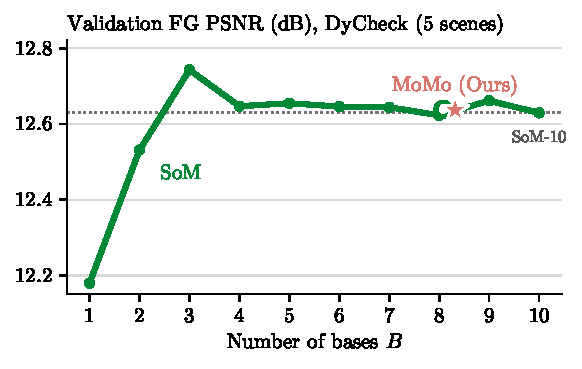
\includegraphics[width=\linewidth]{img/sweep_val_dycheck.pdf}\phantomsubcaption\label{fig:sweep-avg-dycheck}\end{subfigure}\\[2pt]
  \begin{subfigure}{\linewidth}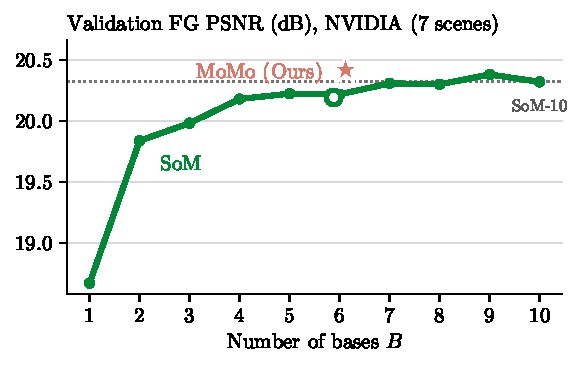
\includegraphics[width=\linewidth]{img/sweep_val_nvidia.pdf}\phantomsubcaption\label{fig:sweep-avg-nvidia}\end{subfigure}
  \caption{\claudetag\ Foreground PSNR on the held-out views against the number of bases, averaged over the five DyCheck
    (iPhone) scenes (top) and the seven NVIDIA scenes (bottom): SoM~\cite{wang2025shape} with $B = 1$--$10$ bases (curve), ours at
    the mean of the $B$ its stopping rule picks per scene (star; 8.2 on DyCheck, 6.0 on NVIDIA) and SoM given each scene's $B$
    (circle); dotted line: SoM-10. Seed 42.}
  \label{fig:sweep-avg}
\end{figure}
 (user request); the old copy's \input is commented out and its text
% struck, with \Cref written as Fig.~\ref because \sout cannot process \cref.
% % [Claude] 2026-10-28: placeholder for the motion-coefficient comparison (user request); grey boxes stand in for the images.
% [Claude] 2026-11-05 (user requests): apple (seed 44), Balloon1 (seed 43) and teddy (seed 43) at the first training frame (0_00000), spin (seed 42)
% at training frame 0_00270 (18 s into the 15 fps render). Coefficients = that frame of tests/render_coefs.py's renders (outputs/bdf/modes_vis/
% {som/<S>/bases_10,split_init/<S>/bases_<B>}[_s<seed>]/videos/epoch_0499/motion_coefs.mp4, right half); input = the dataset's training image,
% cropped like the render (Balloon1: 458 x 240 of 470 x 248; DyCheck 720 x 960, uncropped).
\begin{figure}[t]
  \centering
  \newcommand{\coefrow}[3]{\rotatebox{90}{\makebox[#2\linewidth][c]{\footnotesize #3}} & \coefimg{coef_#1_input} & \coefimg{coef_#1_som10} &
    \coefimg{coef_#1_ours} \\}
  \newcommand{\coefimg}[1]{\includegraphics[width=0.3\linewidth]{img/#1}}
  \setlength{\tabcolsep}{1pt}
  \begin{tabular}{@{}c@{\hspace{2pt}}ccc@{}}
    \coefrow{apple_s44_f0}{0.4}{Apple}
    \coefrow{Balloon1_s43_f0}{0.157}{Balloon1}
    \coefrow{teddy_s43_f0}{0.4}{Teddy}
    \coefrow{spin_s42_f270}{0.4}{Spin}
     & \makebox[0.3\linewidth][c]{\footnotesize Input} &
       \makebox[0.3\linewidth][c]{\footnotesize SoM-10} &
       \makebox[0.3\linewidth][c]{\footnotesize Ours} \\
  \end{tabular}
  \caption{\claudetag\ Motion coefficients of Shape of Motion~\cite{wang2025shape} with its default 10 bases and of our method
    ($B$ from its stopping rule: 5 on apple, 4 on Balloon1, 8 on teddy, 9 on spin), rendered from a training view: the first one for
    apple (DyCheck, seed 44), Balloon1 (NVIDIA, seed 43) and teddy (DyCheck, seed 43), frame 270 for spin (DyCheck, seed 42). Each
    foreground Gaussian is coloured by its blending weights: every basis of a model has its own hue, spaced evenly over that model's
    bases, and mixed weights mix the hues; the background is grey. Hues are not matched between the two methods: what matters is which
    parts share one colour.}
  \label{fig:coef-comparison}
\end{figure}


% \begin{figure}[t]
  \centering
  \begin{subfigure}[b]{0.48\linewidth}
    \centering
    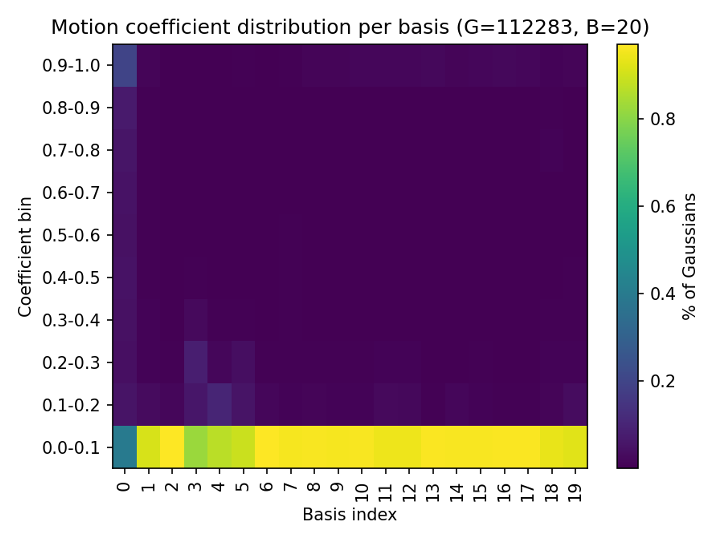
\includegraphics[width=\linewidth]{img/basis_distribution_ours.png}
    \caption{Ours}
    \label{fig:basis-distribution-ours}
  \end{subfigure}
  \hfill
  \begin{subfigure}[b]{0.48\linewidth}
    \centering
    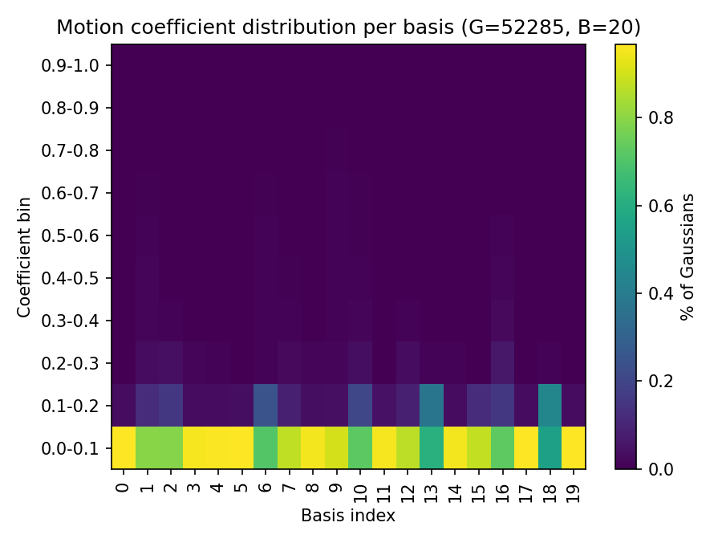
\includegraphics[width=\linewidth]{img/basis_distribution_som.png}
    \caption{Shape-of-Motion}
    \label{fig:basis-distribution-som}
  \end{subfigure}
  \caption{Distribution of motion basis coefficients after softmax. }
  \label{fig:basis-distribution}
\end{figure}

% Figure~\ref{fig:basis-distribution} shows that the motion bases coefficients trained using our method concentrate around the first basis at initialization, and the remaining bases are mostly used for local correction.
% In comparison, Shape-of-Motion~\cite{wang2025shape}'s coefficients are uniformly distributed among all bases.

% Our method solves the issue of object deformations that Shape-of-Motion exhibits.
% Our method shows a much closer alignment with the ground truth global orientation of the object.
% This is because our method emphasizes the global object orientation and position, as shown in the motion bases coefficients analysis in Fig.~\ref{fig:basis-distribution}.

% Figure~\ref{fig:qualitative-comparison} presents qualitative results on the Apple, Paper Windmill, and Teddy scenes, comparing our rendered novel views and estimated tracks against the ground truth and Shape-of-Motion~\cite{wang2025shape}.


